\gls{atlas} is a multi purpose detector designed to be sensitive to a large
physics signatures (supersymmetry, dark matter and extra dimensions) and to
fully take advantage of the LHC potential. It is capable of identifying photons,
electrons, muons, taus, jets and missing energy,
Figure~\ref{fig:atlas_particles} shows a schematic view of the interaction of
the different kind of particles with the ATLAS sub-detectors while
Figure~\ref{fig:atlas_overview} shows the ATLAS detector with its subsystems. In
the following sections a brief overview of the various system that allow
particle identification and reconstruction is presented.

\begin{figure}[!h]
  \centering
  \begin{subfigure}[t]{.48\linewidth}
    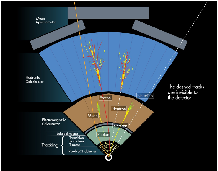
\includegraphics[width=\linewidth]{atlas_particles}
    \caption{Section of the ATLAS detector showing the interaction of different
      particles with the sub-detectors.}
    \label{fig:atlas_particles}
  \end{subfigure} \quad
  \begin{subfigure}[t]{.48\linewidth}
    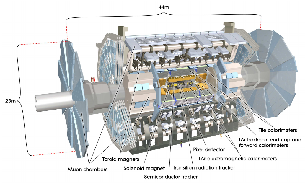
\includegraphics[width=\linewidth]{atlas_overview}
    \caption{Overview of the ATLAS detectors with its main sub-detectors.}
    \label{fig:atlas_overview}
  \end{subfigure}
  \caption{}
  \label{fig:atlas}
\end{figure}
%%% Local Variables:
%%% mode: latex
%%% TeX-master: "../search_for_DM_LED_with_ATLAS"
%%% End:
